\documentclass[12pt]{extarticle}
\usepackage[utf8]{inputenc}
\usepackage{amsmath}
\usepackage{hyperref}
\usepackage[shortlabels]{enumitem}
\usepackage{tikz}
\usepackage{textcomp}

\addtolength{\textwidth}{1.0in}
\addtolength{\textheight}{0.75in}
\addtolength{\evensidemargin}{-0.75in}
\addtolength{\oddsidemargin}{-0.75in}
\addtolength{\topmargin}{-1.0in}

\title{Circle Geometry - Answers}
\author{Eric Xiao}
\date{April 18, 2020}

\usepackage{natbib}
\usepackage{graphicx}

\begin{document}

\maketitle

\section{Problems}
\begin{enumerate}
    \item {In the following circle, points A and B lie on its circumference, while point O is an arbitrary point inside the circle. What is the value of \angle ABO?\\
    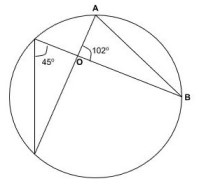
\includegraphics{April_18_Q1} Answer: \fbox{33\textdegree}}
    \item {In the circle below with center O, points L, M, and N lie on its circumference. If \angle MON = {98\textdegree} and \angle LMO = {40\textdegree}, what is the value of \angle LNO?\\
    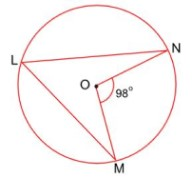
\includegraphics{April_18_Q2} Answer: \fbox{9\textdegree}}
    \item {In the diagram below, side lengths RS and RT are tangent to the circle with centre O, and U is a point on its circumference. If \angle SRT = {40\textdegree}, find the value of \angle SUT.\\
    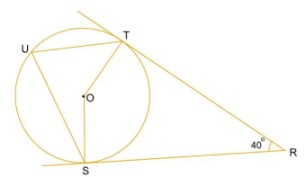
\includegraphics{April_18_Q3} Answer: \fbox{70\textdegree}}
    \item {In the diagram below, ABC is a triangle whose side lengths are all tangents to a circle with centre O. AB intersects the circle at D, BC at E, and AC at F. If AD = 10, BE = 4, CF = 5, and circle O's radius is 3, what is the area of triangle ABC?\\
    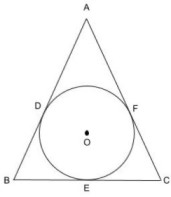
\includegraphics{April_18_Q4} Answer: \fbox{57}}
    \item {In the circle below, CD is the diameter and AB is a chord. Both side lengths intersect perpendicularly at point E. If AB = $\sqrt{800}$, DE = {$a$}, and CE = {$8a$}, find the radius of the circle.\\
    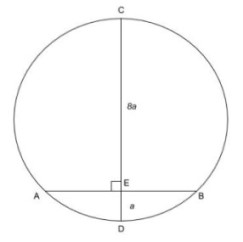
\includegraphics{April_18_Q5} Answer: \fbox{$\frac{45}{2}$ or 22.5}}
\end{enumerate}
\end{document}